\scanpage{119}
\mspage{59}

that of a universal covering \deleted{\unsure{(précis.|(precis.}} \inserted{or again} of a geometric point $\unsure{\zeta|\xi}$ of $\unsure{\widetilde K_x|\widetilde U_x}$ --- i.e. of an algebraic closure of $\widetilde K_x$ --- \uline{and} of a \deleted{\unsure{isomorphism}} ``path of domains'' between $\unsure{\zeta|\xi}_{\widetilde U_x}\longrightarrow\unsure{\widetilde K_x|\widetilde U_x}\longrightarrow\operatorname{Spec}(L)$ and $\unsure{\zeta|\xi}_L$ defined by $\widetilde L$ --- or what amounts to the same, \inserted{up to isomorphism of the \unsure{coverings|lifts}} of an $\deleted{\unsure{K}}L$-homomorphism from \deleted{$\unsure{K_x|K}$} \deleted{$\unsure{K_x|K}$} $\widetilde L_x$ into $\overline L$ --- and this in turn is equivalent to the datum of an $x'$, \deleted{\uline{and} of an isomorphism} as above. This being so, we have canonical isomorphisms.

\[
(30)\quad\left\{\begin{aligned}
N_{x'}&\simeq\mathcal E_{\widetilde U_x}^{\overline L}\\
I_{x'}&\simeq\text{Kernel of the canonical homomorphism }\inserted{\text{surjective}}\\
&\mathcal E_{\widetilde U_x}^{\overline L}\longrightarrow\mathcal E_{\overline{k(x)}}
\end{aligned}\right.
\]
(where the \inserted{algebraic} closure $\overline{k(x)}$ of $k(x)$ is induced by the algebraic closure $\overline L$ of $\widetilde K_x$)

\margin{Cf Galois theory\\
of henselian traits\\
here $I_{x'}$ plays the role\\
of a $\unsure{\Pi|\pi}_{\widetilde U_x/k(x)}^{\overline L}$ ; in fact\\
it is $=\unsure{\Pi|\pi}_{\widetilde U_x/\widetilde S_x}^{\overline L}$ !}

(\unsure{Then} (27) is deduced by Kummer theory)\unsure{,}

\deleted{$I_{x'}\unsure{\simeq|=}$}

\deleted{(27)}

\margin{\raisebox{21mm}{?}\hspace{5mm}%
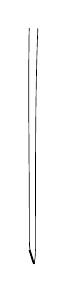
\begin{tikzpicture}[x=1mm,y=1mm,baseline=0pt]
\draw[line width=0.25pt] (0,30) .. controls (-0.15,21) and (0.05,11) .. (0.02,3) .. controls (0.02,1.7) and (0.28,0.8) .. (0.62,0.05);
\draw[line width=0.23pt] (1.1,30) .. controls (0.73,21) and (0.82,10) .. (0.78,2.3) .. controls (0.84,1) and (0.68,0.45) .. (0.62,0.05);
\draw[line width=0.65pt] (0.04,1.8) .. controls (0.25,1.25) and (0.42,0.5) .. (0.62,0.05);
\end{tikzpicture}}
I presume that (in the present situation --- or even, with a base field $K$) we have $N_{x'}=\operatorname{Norm}_{\mathcal E_L}(I_{x'})$, \inserted{(a priori, we only have $\subset$)} which is linked to the idea that we should have $I_{x'}=\operatorname{Norm}_{\unsure{\Pi|\pi}_{L/K}}(I_{x'})$

\margin{118}
